\documentclass[a4paper,12pt]{article}
\usepackage[T1]{fontenc}

\usepackage{graphicx} 
\usepackage{float}
\usepackage{wrapfig} 
\input{epsfx}

\usepackage[utf8]{inputenc}
\usepackage{polski}
\prefixing

\setlength{\parindent}{20pt}

%\author{Przemysław Woldon}
%\date{}

\begin{document}
	\title{PRACA DYPLOMOWA INŻYNIERSKA}
	\maketitle
	\pagenumbering{gobble}
	
	\newpage
	
	\pagenumbering{arabic}
	\setcounter{page}{2}
	\section*{Streszczenie}
	\section*{Abstract}

	\newpage 

	\section{Wstęp}
		\subsection{Motywacja wyboru pracy}
			\paragraph{\noindent} 
				Obecnie coraz częściej w kościo\l ach czy świątyniach możemy spotkać rzutniki czy wyświetlacze led, na których ekranizowane są teksty pieśni.
				Zbiory pieśni dostarczane przez producentów wyświetlaczy nie są w stanie sprostać dynamicznemu rozwojowi muzyki - powstawaniu nowych utworów
				oraz bardzo zróżnicowanym tradycjom lokalnym oraz indywidualnym upodobaniom muzyków kościelnych wykorzystującym różne śpiewniki.
				Czasochłonny proces budowy wspomnianych zbiorów często opiera się na ręcznym przepisywaniu tekstów ze śpiewników.
				Automatyzacja tego procesu pozwoli na łatwiejsze dopasowanie zbiorów do potrzeb muzyków kościelnych i tradycji lokalnych. 

		\subsection{Cel pracy}
			\paragraph{\noindent}
				Podjęte wysiłki miały na celu zaprojektowanie algorytmów oraz budowę aplikacji okienkowej o prostym i przyjaznym dla użytkownika interfejsie, która umożliwi pozyskanie ze zdjęć śpiewników tekstów pieśni.
				Opierając się na przetwarzaniu obrazów (detekcji i usunięciu znaków muzycznych) i rozpoznawaniu ciągów znaków abecadła (słów) uwzględniając polskie znaki diakrytyczne.

	\newpage 

	\section{Wykorzystane technologie}
		\subsection{Biblioteka OpenCv}
			\paragraph{\noindent} 
				OpenCv jest biblioteką s\l użącą do komputerowego przetwarzania obrazów oraz uczenia maszynowego, 
				o otwartym kodzie źród\l owym.
		\subsubsection{Zarys historyczny}
			\paragraph{\noindent} 
				Prace nad budową tej biblioteki rozpoczął jeden z pracowników firmy Intel - Gary Rost Bradski, zainspirowany środowiskiem akademickim, które wówczas posiadało bardzo bogatą infrastrukturę służącą do przetwarzania obrazów, jednak przeznaczoną dla użytku wewnętrznego. 
				Studenci w obrębie jednej jednostki akademickiej dzielili się kodem zawierającym gotowe implementacje algorytmów, co znacząco ułatwiało prace przy własnych projektach czy aplikacjach. 
				Stąd głównym celem biblioteki OpenCv jest udostępnienie wszystkim zainteresowanym zagadnieniami przetwarzania obrazów i sztucznej inteligencji gotowej jednolitej, darmowej infrastruktury pozwalającej na pracę, tak aby nie trzeba było ponownie ''wynajdywać koła''.

			\paragraph{\noindent}  
				OpenCv zostało przedstawione po raz pierwszy w 1999 roku szerszemu gronu odbiorców. 
 
			\paragraph{\noindent Wersja 1.0}
				W wersji 1.0 kod biblioteki stanowiły wyłącznie najbardziej użyteczne przy przetwarzaniu obrazów
				algorytmy zaimplementowane w języku C. 
				Od tego czasu biblioteka znacząco się zmieniła. 
			\paragraph{\noindent Wersja 2.0}
				W wersji 2.0 znaczący wpływ na wydanie wywarły trendy obecne w prowadzeniu projektów, w których wytwarza się oprogramowanie - repozytorium kodu w systemie kontroli wersji Git, gdzie możemy znaleźć najnowszą wersję biblioteki i najświeższe poprawki, testy jednostkowe czy booty ciągłej kompilacji. 
				Zaimplementowano również interfejsy dla języków programowania takich jak C++ oraz Javy, Python’a, MATLAB-a.
				Od tego czasu nowe typy danych i funkcje metody implementowano w C++, a już napisane w języku C dopasowano do nowej technologii.
			\paragraph{ \noindent Wersja 3.0}
				Nieustannie zwiększająca się liczba zaimplementowanych algorytmów użytecznych przy przetwarzaniu obrazów przyczyniła się do modułowej budowy biblioteki w wersji 3.0, która przedstawia się w sposób następujący:


				\begin{enumerate}
					\item (Warstwa wierzchnia) system operacyjny,
					\item interfejsy dla różnych języków i aplikacje,
					\item moduł \textit {opencv\_contrib} zawierający kod napisany i dołączony do biblioteki przez użytkowników,
					\item rdzeń OpenCv,
					\item optymalizacje sprzętowe (warstwa HAL \textit {ang. hardware acceleration layer}).
				\end{enumerate} 

				\begin{figure}[!ht]   %Srodowisko do umieszczania rysunkow
					\begin{center}
						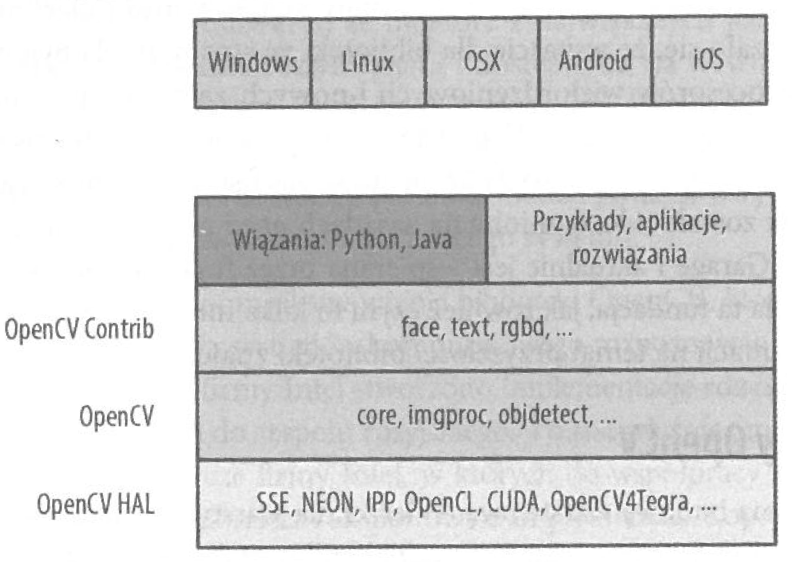
\includegraphics[width=10cm] {budowaModulowa.png} 
					\end{center}
					\caption
					[Budowa modułowa OpenCv]  % Podpis - do spisu tresci
					{Budowa modułowa OpenCv}  %Podpis
				\end{figure}

				OpenCv w tej wersji wspiera budowanie i dołączanie do biblioteki walsnych modulów.

	\newpage
				\begin{figure}[!ht]   %Srodowisko do umieszczania rysunkow
					\begin{center}
						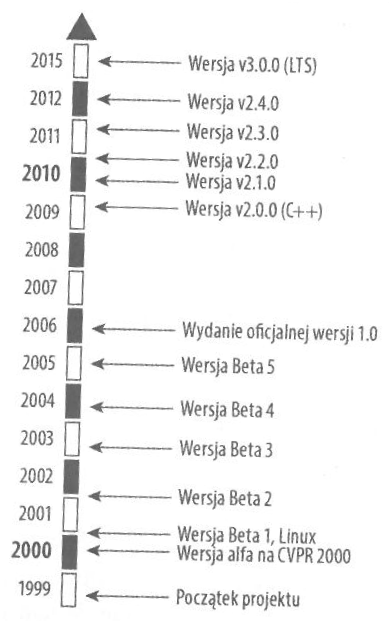
\includegraphics[width=7cm] {osCzasu.png} 
					\end{center}
					\caption
					{Rozwój projektu w czasie}  %Podpis
					[Rozwój projektu w czasie]  % Podpis - do spisu tresci
				\end{figure}


		\subsubsection{Popularność projektu}  
			\paragraph{\noindent}
				Projekt cieszy się bardzo dużym powodzeniem, które nieustannie rośnie. Świadczy o tym liczba pobrań 
				wynosząca około 14 milionów razy, zaś miesięcznie około 200 tysięcy.
				Obecnie biblioteka zawiera ponad 2500 zoptymalizowanych algorytmów, które służą do przetwarzania obrazów
				również w czasie rzeczywistym i uczenia maszynowego, co znacząco ułatwia tworzenie aplikacji użytkownikom. 
				Programiści piszący kod uwzględniali wymóg przenośności OpenCv, a więc możliwości kompilacji na każdym odpowiednim kompilatorze języka C++, co wymusiło restrykcyjną zgodność ze standardem i ułatwiło obsługę różnych platform.
				Biblioteka dostępna jest na systemach operacyjnych takich jak: Windows, Linux, Mac OS X, do których dołączyły systemy operacyjne platforma mobilnych (Android i IOS), co znacząco przyczyniło się do zwiększenia liczby użytkowników

		\subsubsection{Zastosowania biblioteki OpenCv}
			Dynamiczny rozwój technologiczny otwiera przed biblioteką nowy horyzont użyteczności.
			OpenCv znajduje zastosowanie w wielu obszarach życia do tego stopnia że wykorzystanie projektu wydaje się rzeczą całkowicie naturalna a wręcz niezauważalną. Biblioteka wykorzystywana jest w:
			\begin{itemize}
				\item skanowaniu kodów QR,
				\item monitoringu,
				\item rozpoznawaniu dzwięków i muzyki,
				\item obrazowaniu medycznym,
				\item robotyce,	
				\item przemyśle - produkcji masowej i kontroli jakości,
				\item wojsku - bezzałogowe pojazdy, fotografie lotnicze,
				\item analizie obiektów,
				\item Google Street View,
			\end{itemize}

	
	\subsection{Formaty obrazow}
		\textbackslash\textbackslash
		obrazy kolorowe i w skali szrosci\\
		\textbackslash\textbackslash
		jpg jak przechowuwany w pamieci budowa pixeli bitowo

	\subsection{Język programowania Java SE 8}
		\textbackslash\textbackslash wstep o jezyku \\
		\textbackslash\textbackslash popularnosc co pomoze w utrzymaniu projektu \\
		\textbackslash\textbackslash lambdy i strumienie ulatwiajace przetrwarzane


	\subsection{Eclipse}
		\textbackslash\textbackslash
		srodowisko i kofiguracja


\section{Część praktyczna}
	\subsection{Budowa aplikacji}
		Algorytmy przetwarzające obrazy zosta\l y umieszczone w odpowiednich klasach, u\l atwiających pos\l ugiwanie się nimi. Rozwiązanie to wychodzi na przeciw podstawowym zasadą obiektowości takim jak: modularyzacja, hermentyzacja, abstrakcja. W aplikacji możemy wyróżnić następujące kalsy: 
		\begin{enumerate}
			\item GetImgFromPdf --- ekstrakscja stron z pliku pdf do obrazów( jedna strona pliku pdf odpowiada jednemu obrazowi);
			\item ImproveImg --- polepszenie jakości obrazu;
			\item CutBlackArea --- usunięcie z obrazu obszarów które nie należą do stron;
			\item DivideToPage --- podzia\l obrazu na dwie strony;
			\item ToStraightenUp --- wyprostowanie obrazu;
			\item MajorProcessing --- zasadnicze przetwarzanie obrazu, detekcja obszarów zawierających znaki muzyczne i teksty; 
			\item DetectText --- wykrycie i ''odczytanie'' tekstu; 
			\item PrepareImgToAnalize --- przygotowanie obrazu do analizy poprzez budowę zbiorów lini.
		\end{enumerate} 

		\subsubsection{Klasa GetImgFromPdf}
			Przy pomocy biblioteki Apache PDFBox do\l ączonej do projektu jako plik z rozszerzeniem jar, z plików pdf pobieramy strony konwertujac je do kolorowych plików graficznych z określoną rozdzielczością.
	
			ALGORYTM
			
		\subsubsection{Klasa CutBlackArea}
			Wycięcie z obrazu czarnych obszarów, które są uzupe\l nieniem interesujących nas zakresów stron do określonego formatu skanu. Algorytm wykorzystuje do tego wartości odchylenia standardowego w poziomych liniach obrazu i wartości dominanty. Przy założeniu, że te powierzchnie znajdują się po lewej stronie i na dole obrazu. Algorytm umożliwia wycięcie jednego( dolnego) lub obu obszarów. 
			
			ALGORYTM\\
			WYKRES z StdDev
			
			Na podstawie wykresu widzimy, że wiersze obrazu( w skali szarości) o ma\l ej zmienności wartości pikseli, będą dawa\l y niewielkie wartości odchylenia standardwego. Jeśli nie równa się ono zeru, ale jest odpowiednio ma\l e możemy za\l ożyć, że badany wiersz ma jedną barwę, a wartość ta wynika z drobnych zak\l uceń i niedoskona\l ości obrazu.
			
			Do obliczenia odchylenia standardowego została użyta funkcja udostępniona w bibliotece OpenCv:\\ 
			\textit {Core.meanStdDev(Mat src, MatOfDouble mean, MatOfDouble stddev)}.\\
			Oblicza ona średnią i odchylenie standardowe macieży podanej jako parametr src( w algorytnie jest to jeden wiersz obrazu), które zależy od wszystkich kanałów macieży. Tutaj jest to jeden kanał --- obraz przed obliczeniami został prztransformowany do skali szarości według poniższego algorytmu:
			 
						
			Za obliczenie wartości najczęściej występującej odchylenia standardowego odpowiada funkcja: \\
			\textit {public List \guilsinglleft Double\guilsinglright calculateModeOfStdDev(List \guilsinglleft Double\guilsinglright stdDevList)}\\
			wykorzystująca nowe rozwiązania wprowadzone w Javie wersji 8, a więc strumienie i wyrażenia lambda, co znacząco przyśpiesza czas obliczeń oraz przejrzystość napisanego kodu. 
			
			
		

\end{document}